         \chapter{Analytical geometry}
    \setcounter{figure}{1}
    \setcounter{subfigure}{1}
    \label{71522cd1c95e0cbedb9f300409036b1b}
    
    
    
    
       
%          \section{ Cartesian plane \& Distance between two points}
%     \nopagebreak
%             \label{m39107} $ \hspace{-5pt}\begin{array}{cccccccccccc}   
\includegraphics[width=0.75cm]{col11306.imgs/summary_video.png} &   \end{array} $ \hspace{2 pt}\raisebox{-5 pt}{} {(section shortcode: MG10107 )} \par 
%     
%     
%     
%     
    
    
%   
%       \label{m39107*uid36}
%             \subsection{ Introduction}
%             \nopagebreak
%             
        
        \label{m39107*id66769}Analytical geometry, also called co-ordinate geometry and earlier referred to as Cartesian geometry, is the study of geometry using the principles of algebra, and the Cartesian co-ordinate system. It is concerned with defining geometrical shapes in a numerical way, and extracting numerical information from that representation. Some consider that the introduction of analytic geometry was the beginning of modern mathematics.\par 
      
      \label{m39107*eip-448}
            \section{ Drawing figures on the Cartesian plane}
            \nopagebreak
            \label{m39107*eip-728}If we are given the co-ordinates of the vertices of a figure then we can draw that figure on the Cartesian plane. For example take quadrilateral ABCD with co-ordinates: A(1,1), B(1,3), C(3,3) and D(1,3) and represent it on the Cartesian plane. This is shown in Figure~15.1.   
\par \label{m39107*eip-199}
    \setcounter{subfigure}{0}


	\begin{figure}[H] % horizontal\label{m39107*id63458}
    \begin{center}
    \label{m39107*id63458!!!underscore!!!media}\label{m39107*id63458!!!underscore!!!printimage}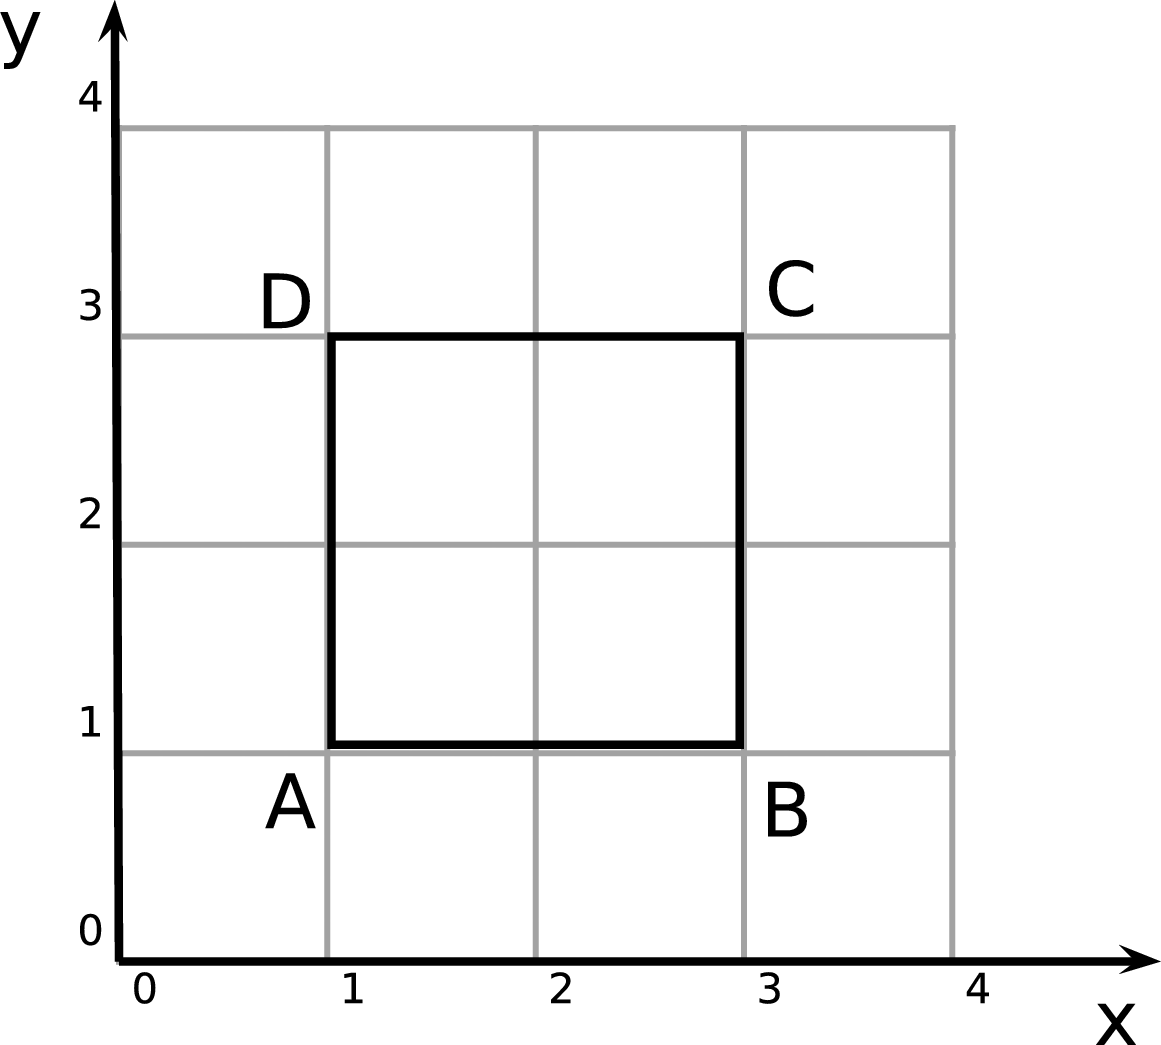
\includegraphics[width=300px]{col11306.imgs/m39107_square.png} % m39107;square.png;;;6.0;8.5;
        
      \vspace{2pt}
    \vspace{\rubberspace}\par \begin{cnxcaption}
	  \small \textbf{Figure 15.1: }Quadrilateral ABCD represented on the Cartesian plane
	\end{cnxcaption}
      
    \vspace{.1in}
    
    \end{center}

 \end{figure}   

    \addtocounter{footnote}{-0}
    
\par \label{m39107*eip-645}To represent any figure on the Cartesian plane, you place a dot at each given co-ordinate and then connect these points with straight lines. One point to note is in naming a figure. In the above example, we called the quadrilateral ABCD. This tells us that we move from point A, to point B, to point C, to point D and then back to point A again. So when you are asked to draw a figure on the Cartesian plane, you will follow this naming scheme. If you had the same points, and called it, for example, ACBD you would not get a quadrilateral but a pair of triangles instead. This is important. Sometimes you may be given only some of the points and you will then be required to find the other points using the work covered in the rest of this chapter. \par \label{m39107*uid37}
            \section{ Distance between Two Points}
            \nopagebreak
            \label{m39107*id66786}One of the simplest things that can be done with analytical geometry is to calculate the distance between two points. \textsl{Distance} is a number that describes how far apart two point are. For example, point \begin{math}P\end{math} has co-ordinates \begin{math}\left(2,1\right)\end{math} and point \begin{math}Q\end{math} has co-ordinates \begin{math}\left(-2,-2\right)\end{math}. How far apart are points \begin{math}P\end{math} and \begin{math}Q\end{math}? In the figure, this means how long is the dashed line?\par 
        
    \setcounter{subfigure}{0}


	\begin{figure}[H] % horizontal\label{m39107*uid38}
    \begin{center}
    \rule[.1in]{\figurerulewidth}{.005in} \\
        \label{m39107*uid38!!!underscore!!!media}\label{m39107*uid38!!!underscore!!!printimage}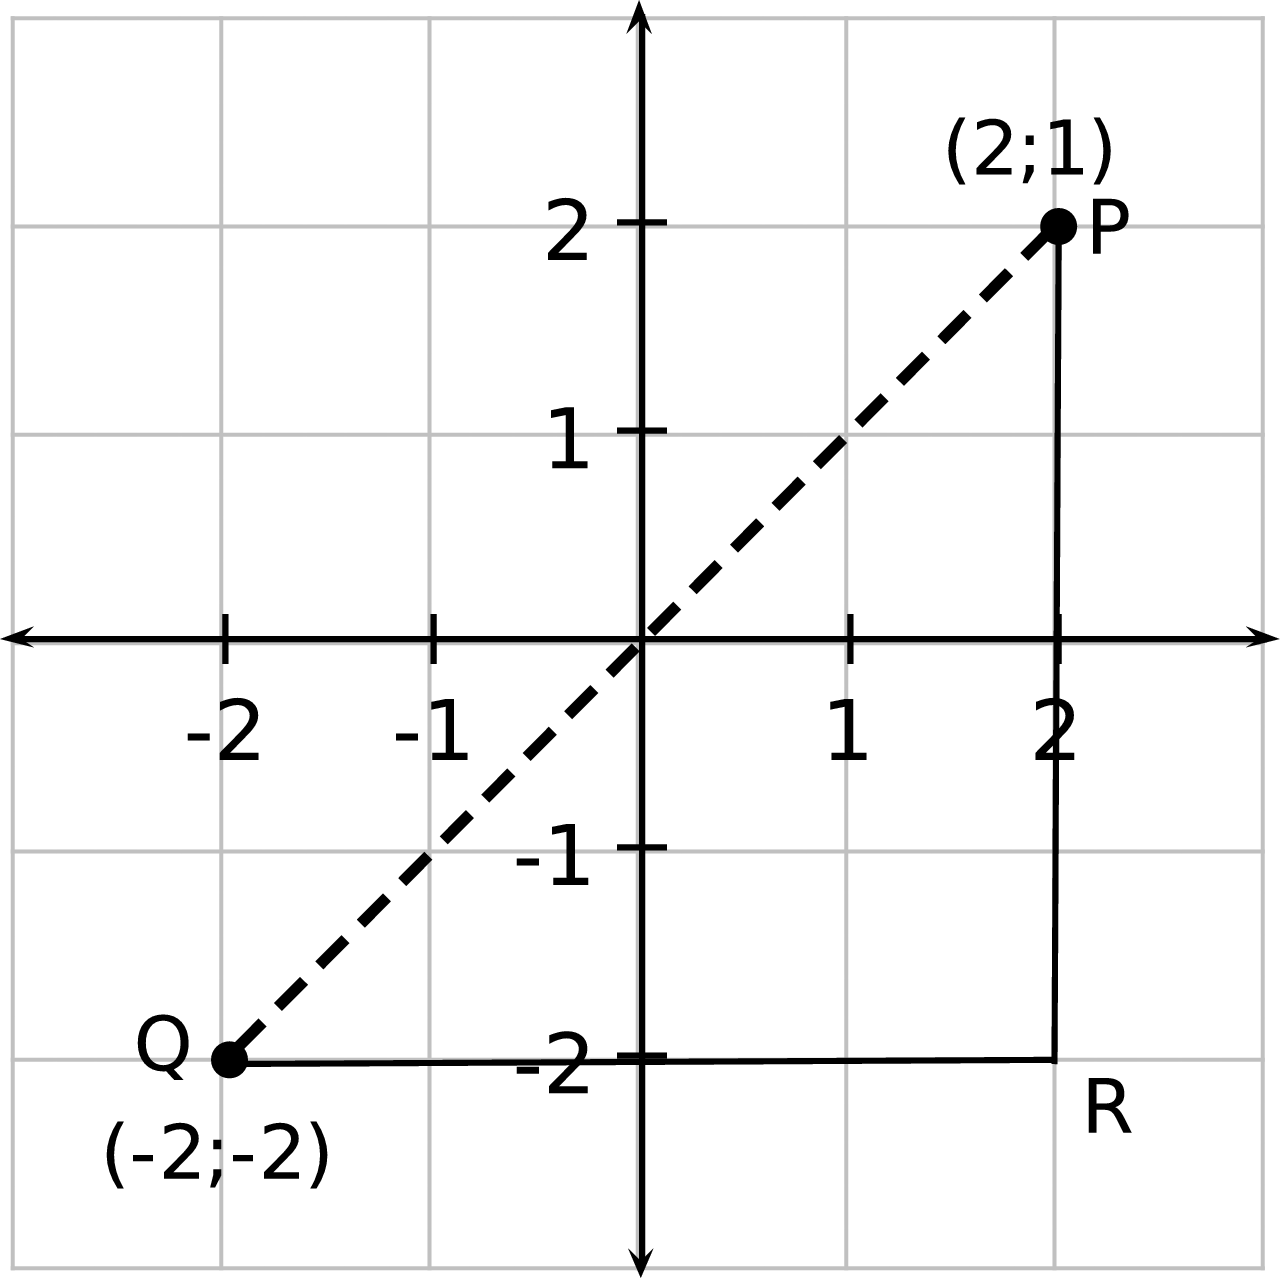
\includegraphics{col11306.imgs/m39107_MG10C14_015.png} % m39107;MG10C14\_015.png;;;6.0;8.5;
        
      \vspace{2pt}
    \vspace{.1in}
    \rule[.1in]{\figurerulewidth}{.005in} \\
        
    \end{center}

 \end{figure}   

    \addtocounter{footnote}{-0}
    
        \label{m39107*id66883}In the figure, it can be seen that the length of the line \begin{math}PR\end{math} is 3 units and the length of the line \begin{math}QR\end{math} is four units. However, the \begin{math}\mathrm{\^{a}--µ}PQR\end{math}, has a right angle at \begin{math}R\end{math}. Therefore, the length of the side \begin{math}PQ\end{math} can be obtained by using the Theorem of Pythagoras:\par 
        \label{m39107*id66950}\nopagebreak\noindent{}
          \settowidth{\mymathboxwidth}{\begin{equation}
    \begin{array}{ccc}\hfill P{Q}^{2}& =& P{R}^{2}+Q{R}^{2}\hfill \\ \hfill \^{a}ˆ´P{Q}^{2}& =& {3}^{2}+{4}^{2}\hfill \\ \hfill \^{a}ˆ´PQ& =& \sqrt{{3}^{2}+{4}^{2}}=5\hfill \end{array}\tag{15.1}
      \end{equation}
    }
    \typeout{Columnwidth = \the\columnwidth}\typeout{math as usual width = \the\mymathboxwidth}
    \ifthenelse{\lengthtest{\mymathboxwidth < \columnwidth}}{% if the math fits, do it again, for real
    \begin{equation}
    \begin{array}{ccc}\hfill P{Q}^{2}& =& P{R}^{2}+Q{R}^{2}\hfill \\ \hfill \^{a}ˆ´P{Q}^{2}& =& {3}^{2}+{4}^{2}\hfill \\ \hfill \^{a}ˆ´PQ& =& \sqrt{{3}^{2}+{4}^{2}}=5\hfill \end{array}\tag{15.1}
      \end{equation}
    }{% else, if it doesn't fit
    \setlength{\mymathboxwidth}{\columnwidth}
      \addtolength{\mymathboxwidth}{-48pt}
    \par\vspace{12pt}\noindent\begin{minipage}{\columnwidth}
    \parbox[t]{\mymathboxwidth}{\large\begin{math}
    P{Q}^{2}=P{R}^{2}+Q{R}^{2}\^{a}ˆ´P{Q}^{2}={3}^{2}+{4}^{2}\^{a}ˆ´PQ=\sqrt{{3}^{2}+{4}^{2}}=5\end{math}}\hfill
    \parbox[t]{48pt}{\raggedleft 
    (15.1)}
    \end{minipage}\vspace{12pt}\par
    }% end of conditional for this bit of math
    \typeout{math as usual width = \the\mymathboxwidth}
    
        
        \label{m39107*id67090}The length of \begin{math}PQ\end{math} is the distance between the points \begin{math}P\end{math} and \begin{math}Q\end{math}.\par 
        \label{m39107*id67126}In order to generalise the idea, assume \begin{math}A\end{math} is any point with co-ordinates \begin{math}\left({x}_{1};{y}_{1}\right)\end{math} and \begin{math}B\end{math} is any other point with co-ordinates \begin{math}\left({x}_{2};{y}_{2}\right)\end{math}.\par 
        
    \setcounter{subfigure}{0}


	\begin{figure}[H] % horizontal\label{m39107*uid39}
    \begin{center}
    \rule[.1in]{\figurerulewidth}{.005in} \\
        \label{m39107*uid39!!!underscore!!!media}\label{m39107*uid39!!!underscore!!!printimage}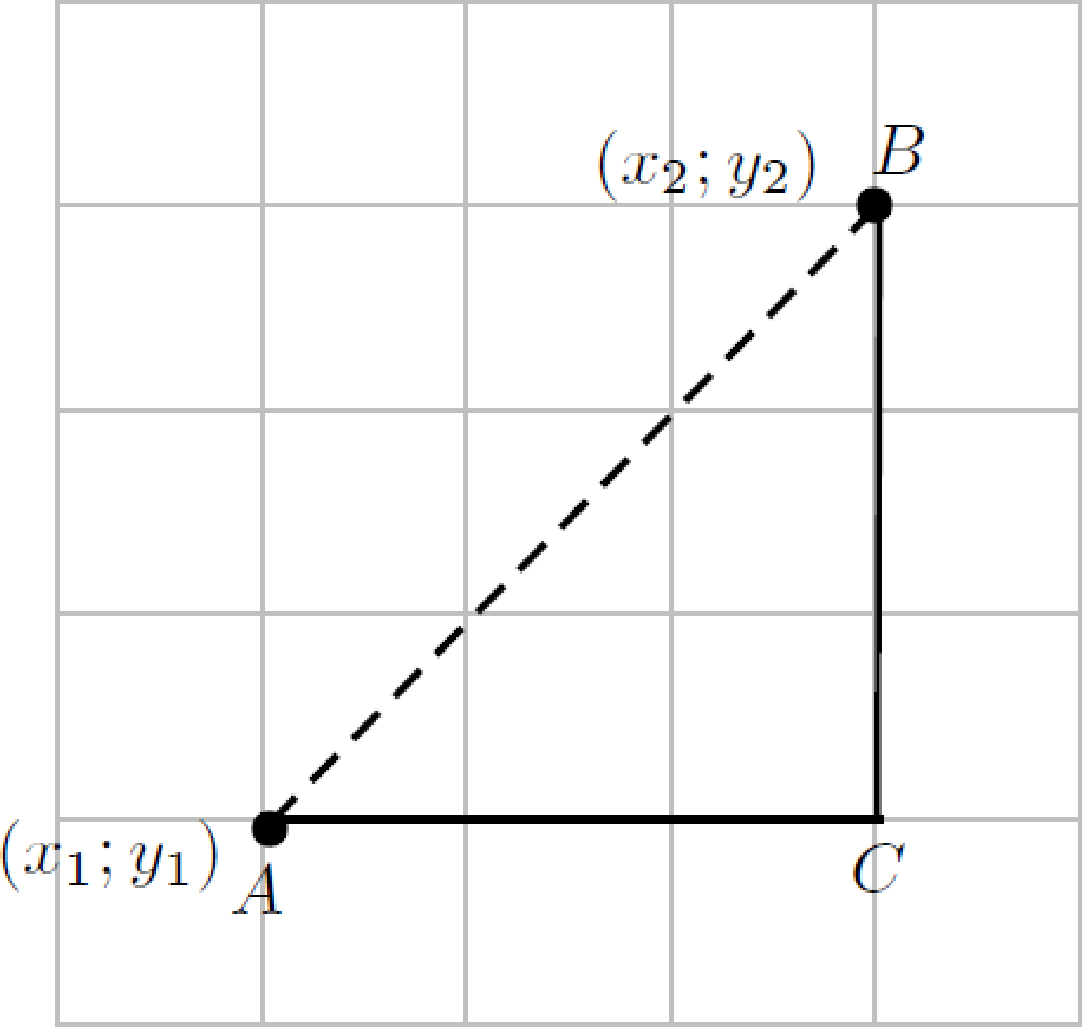
\includegraphics{col11306.imgs/m39107_MG10C14_016.png} % m39107;MG10C14\_016.png;;;6.0;8.5;
        
      \vspace{2pt}
    \vspace{.1in}
    \rule[.1in]{\figurerulewidth}{.005in} \\
        
    \end{center}

 \end{figure}   

    \addtocounter{footnote}{-0}
    
        \label{m39107*id67214}The formula for calculating the distance between two points is derived as follows. The distance between the points \begin{math}A\end{math} and \begin{math}B\end{math} is the length of the line \begin{math}AB\end{math}. According to the Theorem of Pythagoras, the length of \begin{math}AB\end{math} is given by:\par 
        \label{m39107*id67261}\nopagebreak\noindent{}
          \settowidth{\mymathboxwidth}{\begin{equation}
    AB=\sqrt{A{C}^{2}+B{C}^{2}}\tag{15.2}
      \end{equation}
    }
    \typeout{Columnwidth = \the\columnwidth}\typeout{math as usual width = \the\mymathboxwidth}
    \ifthenelse{\lengthtest{\mymathboxwidth < \columnwidth}}{% if the math fits, do it again, for real
    \begin{equation}
    AB=\sqrt{A{C}^{2}+B{C}^{2}}\tag{15.2}
      \end{equation}
    }{% else, if it doesn't fit
    \setlength{\mymathboxwidth}{\columnwidth}
      \addtolength{\mymathboxwidth}{-48pt}
    \par\vspace{12pt}\noindent\begin{minipage}{\columnwidth}
    \parbox[t]{\mymathboxwidth}{\large\begin{math}
    AB=\sqrt{A{C}^{2}+B{C}^{2}}\end{math}}\hfill
    \parbox[t]{48pt}{\raggedleft 
    (15.2)}
    \end{minipage}\vspace{12pt}\par
    }% end of conditional for this bit of math
    \typeout{math as usual width = \the\mymathboxwidth}
    
        
        \label{m39107*id67300}However,\par 
        \label{m39107*id67306}\nopagebreak\noindent{}
          \settowidth{\mymathboxwidth}{\begin{equation}
    \begin{array}{cc}\hfill BC={y}_{2}-{y}_{1}\\ \hfill AC={x}_{2}-{x}_{1}\end{array}\tag{15.3}
      \end{equation}
    }
    \typeout{Columnwidth = \the\columnwidth}\typeout{math as usual width = \the\mymathboxwidth}
    \ifthenelse{\lengthtest{\mymathboxwidth < \columnwidth}}{% if the math fits, do it again, for real
    \begin{equation}
    \begin{array}{cc}\hfill BC={y}_{2}-{y}_{1}\\ \hfill AC={x}_{2}-{x}_{1}\end{array}\tag{15.3}
      \end{equation}
    }{% else, if it doesn't fit
    \setlength{\mymathboxwidth}{\columnwidth}
      \addtolength{\mymathboxwidth}{-48pt}
    \par\vspace{12pt}\noindent\begin{minipage}{\columnwidth}
    \parbox[t]{\mymathboxwidth}{\large\begin{math}
    BC={y}_{2}-{y}_{1}AC={x}_{2}-{x}_{1}\end{math}}\hfill
    \parbox[t]{48pt}{\raggedleft 
    (15.3)}
    \end{minipage}\vspace{12pt}\par
    }% end of conditional for this bit of math
    \typeout{math as usual width = \the\mymathboxwidth}
    
        
        \label{m39107*id67375}Therefore,\par 
        \label{m39107*id67379}\nopagebreak\noindent{}
          \settowidth{\mymathboxwidth}{\begin{equation}
    \begin{array}{ccc}\hfill AB& =& \sqrt{A{C}^{2}+B{C}^{2}}\hfill \\ & =& \sqrt{{\left({x}_{1}-{x}_{2}\right)}^{2}+{\left({y}_{1}-{y}_{2}\right)}^{2}}\hfill \end{array}\tag{15.4}
      \end{equation}
    }
    \typeout{Columnwidth = \the\columnwidth}\typeout{math as usual width = \the\mymathboxwidth}
    \ifthenelse{\lengthtest{\mymathboxwidth < \columnwidth}}{% if the math fits, do it again, for real
    \begin{equation}
    \begin{array}{ccc}\hfill AB& =& \sqrt{A{C}^{2}+B{C}^{2}}\hfill \\ & =& \sqrt{{\left({x}_{1}-{x}_{2}\right)}^{2}+{\left({y}_{1}-{y}_{2}\right)}^{2}}\hfill \end{array}\tag{15.4}
      \end{equation}
    }{% else, if it doesn't fit
    \setlength{\mymathboxwidth}{\columnwidth}
      \addtolength{\mymathboxwidth}{-48pt}
    \par\vspace{12pt}\noindent\begin{minipage}{\columnwidth}
    \parbox[t]{\mymathboxwidth}{\large\begin{math}
    AB=\sqrt{A{C}^{2}+B{C}^{2}}=\sqrt{{\left({x}_{1}-{x}_{2}\right)}^{2}+{\left({y}_{1}-{y}_{2}\right)}^{2}}\end{math}}\hfill
    \parbox[t]{48pt}{\raggedleft 
    (15.4)}
    \end{minipage}\vspace{12pt}\par
    }% end of conditional for this bit of math
    \typeout{math as usual width = \the\mymathboxwidth}
    
        
        \label{m39107*id67499}Therefore, for any two points, \begin{math}\left({x}_{1};{y}_{1}\right)\end{math} and \begin{math}\left({x}_{2};{y}_{2}\right)\end{math}, the formula is:\par 
        \label{m39107*id67561}\begin{math}\mathrm{Distance}=\sqrt{{\left({x}_{1}-{x}_{2}\right)}^{2}+{\left({y}_{1}-{y}_{2}\right)}^{2}}\end{math}\par 
        \label{m39107*id67630}Using the formula, distance between the points \begin{math}P\end{math} and \begin{math}Q\end{math} with co-ordinates (2;1) and (-2;-2) is then found as follows. Let the co-ordinates of point \begin{math}P\end{math} be \begin{math}\left({x}_{1};{y}_{1}\right)\end{math} and the co-ordinates of point \begin{math}Q\end{math} be \begin{math}\left({x}_{2};{y}_{2}\right)\end{math}. Then the distance is:\par 
        \label{m39107*id67728}\nopagebreak\noindent{}
          \settowidth{\mymathboxwidth}{\begin{equation}
    \begin{array}{ccc}\hfill \mathrm{Distance}& =& \sqrt{{\left({x}_{1}-{x}_{2}\right)}^{2}+{\left({y}_{1}-{y}_{2}\right)}^{2}}\hfill \\ & =& \sqrt{{\left(2-\left(-2\right)\right)}^{2}+{\left(1-\left(-2\right)\right)}^{2}}\hfill \\ & =& \sqrt{{\left(2+2\right)}^{2}+{\left(1+2\right)}^{2}}\hfill \\ & =& \sqrt{16+9}\hfill \\ & =& \sqrt{25}\hfill \\ & =& 5\hfill \end{array}\tag{15.5}
      \end{equation}
    }
    \typeout{Columnwidth = \the\columnwidth}\typeout{math as usual width = \the\mymathboxwidth}
    \ifthenelse{\lengthtest{\mymathboxwidth < \columnwidth}}{% if the math fits, do it again, for real
    \begin{equation}
    \begin{array}{ccc}\hfill \mathrm{Distance}& =& \sqrt{{\left({x}_{1}-{x}_{2}\right)}^{2}+{\left({y}_{1}-{y}_{2}\right)}^{2}}\hfill \\ & =& \sqrt{{\left(2-\left(-2\right)\right)}^{2}+{\left(1-\left(-2\right)\right)}^{2}}\hfill \\ & =& \sqrt{{\left(2+2\right)}^{2}+{\left(1+2\right)}^{2}}\hfill \\ & =& \sqrt{16+9}\hfill \\ & =& \sqrt{25}\hfill \\ & =& 5\hfill \end{array}\tag{15.5}
      \end{equation}
    }{% else, if it doesn't fit
    \setlength{\mymathboxwidth}{\columnwidth}
      \addtolength{\mymathboxwidth}{-48pt}
    \par\vspace{12pt}\noindent\begin{minipage}{\columnwidth}
    \parbox[t]{\mymathboxwidth}{\large\begin{math}
    \mathrm{Distance}=\sqrt{{\left({x}_{1}-{x}_{2}\right)}^{2}+{\left({y}_{1}-{y}_{2}\right)}^{2}}=\sqrt{{\left(2-\left(-2\right)\right)}^{2}+{\left(1-\left(-2\right)\right)}^{2}}=\sqrt{{\left(2+2\right)}^{2}+{\left(1+2\right)}^{2}}=\sqrt{16+9}=\sqrt{25}=5\end{math}}\hfill
    \parbox[t]{48pt}{\raggedleft 
    (15.5)}
    \end{minipage}\vspace{12pt}\par
    }% end of conditional for this bit of math
    \typeout{math as usual width = \the\mymathboxwidth}
    
        \label{m39107*eip-130}The following video provides a summary of the distance formula.

    \setcounter{subfigure}{0}


	\begin{figure}[H] % horizontal\label{m39107*uid99}
    
    
    \textnormal{Khan academy video on distance formula}\vspace{.1in} \nopagebreak
  \label{m39107*yt-media}\label{m39107*yt-video}
            \raisebox{-5 pt}{ 
\includegraphics[width=0.5cm]{col11306.imgs/summary_www.png}} { (Video:  MG10108 )}
      
      \vspace{2pt}
    \vspace{.1in}
    
    

 \end{figure}   

    \addtocounter{footnote}{-0}
    \par 
      \label{m39107**end}
          
%          \section{ Calculation of the gradient line}
%     \nopagebreak
%             \label{m39108} $ \hspace{-5pt}\begin{array}{cccccccccccc}   
\includegraphics[width=0.75cm]{col11306.imgs/summary_video.png} &   \end{array} $ \hspace{2 pt}\raisebox{-5 pt}{} {(section shortcode: MG10109 )} \par 
%     
%     
%     
    
    
    
  
      \label{m39108*uid40}
            \section{ Gradient of a line}
            \nopagebreak
            

\label{m39108*id67971}The gradient of a line describes how steep the line is. In the figure, line \begin{math}PT\end{math} is the steepest. Line \begin{math}PS\end{math} is less steep than \begin{math}PT\end{math} but is steeper than \begin{math}PR\end{math}, and line \begin{math}PR\end{math} is steeper than \begin{math}PQ\end{math}.\par 
        
    \setcounter{subfigure}{0}


	\begin{figure}[H] % horizontal\label{m39108*uid41}
    \begin{center}
    \rule[.1in]{\figurerulewidth}{.005in} \\
        \label{m39108*uid41!!!underscore!!!media}\label{m39108*uid41!!!underscore!!!printimage}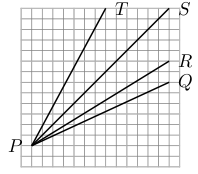
\includegraphics{col11306.imgs/m39108_MG10C14_017.png} % m39108;MG10C14\_017.png;;;6.0;8.5;
        
      \vspace{2pt}
    \vspace{.1in}
    \rule[.1in]{\figurerulewidth}{.005in} \\
        
    \end{center}

 \end{figure}   

    \addtocounter{footnote}{-0}
    
        \label{m39108*id68057}The gradient of a line is defined as the ratio of the vertical distance to the horizontal distance. This can be understood by looking at the line as the hypotenuse of a right-angled triangle. Then the gradient is the ratio of the length of the vertical side of the triangle to the horizontal side of the triangle. Consider a line between a point \begin{math}A\end{math} with co-ordinates \begin{math}\left({x}_{1};{y}_{1}\right)\end{math} and a point \begin{math}B\end{math} with co-ordinates \begin{math}\left({x}_{2};{y}_{2}\right)\end{math}.\par 
        
    \setcounter{subfigure}{0}


	\begin{figure}[H] % horizontal\label{m39108*uid42}
    \begin{center}
    \rule[.1in]{\figurerulewidth}{.005in} \\
        \label{m39108*uid42!!!underscore!!!media}\label{m39108*uid42!!!underscore!!!printimage}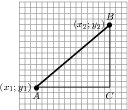
\includegraphics{col11306.imgs/m39108_MG10C14_018.png} % m39108;MG10C14\_018.png;;;6.0;8.5;
        
      \vspace{2pt}
    \vspace{.1in}
    \rule[.1in]{\figurerulewidth}{.005in} \\
        
    \end{center}

 \end{figure}   

    \addtocounter{footnote}{-0}
\subsection{Parallel and Perpendicular Lines}    
        \label{m39108*eip-127}So we obtain the following for the gradient of a line:\par \label{m39108*id68147}\begin{math}\mathrm{Gradient}=\frac{{y}_{2}-{y}_{1}}{{x}_{2}-{x}_{1}}\end{math}\par 
        \label{m39108*eip-332}We can use the gradient of a line to determine if two lines are parallel or perpendicular. If the lines are parallel (Figure~15.7a) then they will have the same gradient, i.e. \begin{math}{m}_{\mathrm{AB}}={m}_{\mathrm{CD}}\end{math}. If the lines are perpendicular (Figure~15.7b) than we have: \begin{math}-\frac{1}{{m}_{\mathrm{AB}}}={m}_{\mathrm{CD}}\end{math}

 
    \setcounter{subfigure}{0}


	\begin{figure}[H] % horizontal\label{m39108*uid4212}
    \begin{center}
    \label{m39108*uid4212!!!underscore!!!media}\label{m39108*uid4212!!!underscore!!!printimage}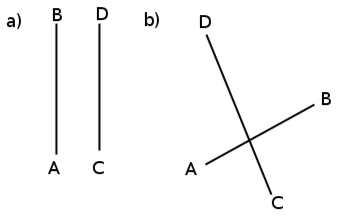
\includegraphics{col11306.imgs/m39108_geom.png} % m39108;geom.png;;;6.0;8.5;
        
      \vspace{2pt}
    \vspace{.1in}
    
    \end{center}

 \end{figure}   

    \addtocounter{footnote}{-0}
    
\par \label{m39108*id68198}For example the gradient of the line between the points \begin{math}P\end{math} and \begin{math}Q\end{math}, with co-ordinates (2;1) and (-2;-2) () is:\par 
        \label{m39108*id68224}\nopagebreak\noindent{}
          \settowidth{\mymathboxwidth}{\begin{equation}
    \begin{array}{ccc}\hfill \mathrm{Gradient}& =& \frac{{y}_{2}-{y}_{1}}{{x}_{2}-{x}_{1}}\hfill \\ & =& \frac{-2-1}{-2-2}\hfill \\ & =& \frac{-3}{-4}\hfill \\ & =& \frac{3}{4}\hfill \end{array}\tag{15.6}
      \end{equation}
    }
    \typeout{Columnwidth = \the\columnwidth}\typeout{math as usual width = \the\mymathboxwidth}
    \ifthenelse{\lengthtest{\mymathboxwidth < \columnwidth}}{% if the math fits, do it again, for real
    \begin{equation}
    \begin{array}{ccc}\hfill \mathrm{Gradient}& =& \frac{{y}_{2}-{y}_{1}}{{x}_{2}-{x}_{1}}\hfill \\ & =& \frac{-2-1}{-2-2}\hfill \\ & =& \frac{-3}{-4}\hfill \\ & =& \frac{3}{4}\hfill \end{array}\tag{15.6}
      \end{equation}
    }{% else, if it doesn't fit
    \setlength{\mymathboxwidth}{\columnwidth}
      \addtolength{\mymathboxwidth}{-48pt}
    \par\vspace{12pt}\noindent\begin{minipage}{\columnwidth}
    \parbox[t]{\mymathboxwidth}{\large\begin{math}
    \mathrm{Gradient}=\frac{{y}_{2}-{y}_{1}}{{x}_{2}-{x}_{1}}=\frac{-2-1}{-2-2}=\frac{-3}{-4}=\frac{3}{4}\end{math}}\hfill
    \parbox[t]{48pt}{\raggedleft 
    (15.6)}
    \end{minipage}\vspace{12pt}\par
    }% end of conditional for this bit of math
    \typeout{math as usual width = \the\mymathboxwidth}
    
        \label{m39108*eip-611}The following video provides a summary of the gradient of a line.

    \setcounter{subfigure}{0}


	\begin{figure}[H] % horizontal\label{m39108*uid993}
    
    
    \textnormal{Gradient of a line}\vspace{.1in} \nopagebreak
  \label{m39108*yt-media1}\label{m39108*yt-video1}
            \raisebox{-5 pt}{ 
\includegraphics[width=0.5cm]{col11306.imgs/summary_www.png}} { (Video:  MG10110 )}
      
      \vspace{2pt}
    \vspace{.1in}
    
    

 \end{figure}   

    \addtocounter{footnote}{-0}
    \par 
      \label{m39108**end}
          
%          \section{ Midpoint of a line}
%     \nopagebreak
%             \label{m39119} $ \hspace{-5pt}\begin{array}{cccccccccccc}   
\includegraphics[width=0.75cm]{col11306.imgs/summary_video.png} &   \end{array} $ \hspace{2 pt}\raisebox{-5 pt}{} {(section shortcode: MG10111 )} \par 
%     
%     
%     
    
    
    
  
      \label{m39119*uid43}
            \section{ Midpoint of a line}
            \nopagebreak
            
        

\label{m39119*id68364}Sometimes, knowing the co-ordinates of the middle point or \textsl{midpoint} of a line is useful. For example, what is the midpoint of the line between point \begin{math}P\end{math} with co-ordinates \begin{math}\left(2;1\right)\end{math} and point \begin{math}Q\end{math} with co-ordinates \begin{math}\left(-2;-2\right)\end{math}.\par 
        \label{m39119*id68433}The co-ordinates of the midpoint of any line between any two points \begin{math}A\end{math} and \begin{math}B\end{math} with co-ordinates \begin{math}\left({x}_{1};{y}_{1}\right)\end{math} and \begin{math}\left({x}_{2};{y}_{2}\right)\end{math}, is generally calculated as follows. Let the midpoint of \begin{math}AB\end{math} be at point \begin{math}S\end{math} with co-ordinates \begin{math}\left(X;Y\right)\end{math}. The aim is to calculate \begin{math}X\end{math} and \begin{math}Y\end{math} in terms of \begin{math}\left({x}_{1};{y}_{1}\right)\end{math} and \begin{math}\left({x}_{2};{y}_{2}\right)\end{math}.\par 
        
    \setcounter{subfigure}{0}


	\begin{figure}[H] % horizontal\label{m39119*uid44}
    \begin{center}
    \rule[.1in]{\figurerulewidth}{.005in} \\
        \label{m39119*uid44!!!underscore!!!media}\label{m39119*uid44!!!underscore!!!printimage}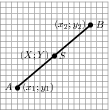
\includegraphics{col11306.imgs/m39119_MG10C14_019.png} % m39119;MG10C14\_019.png;;;6.0;8.5;
        
      \vspace{2pt}
    \vspace{.1in}
    \rule[.1in]{\figurerulewidth}{.005in} \\
        
    \end{center}

 \end{figure}   

    \addtocounter{footnote}{-0}
    
        \label{m39119*id68637}\nopagebreak\noindent{}
          \settowidth{\mymathboxwidth}{\begin{equation}
    \begin{array}{ccc}\hfill X& =& \frac{{x}_{1}+{x}_{2}}{2}\hfill \\ \hfill Y& =& \frac{{y}_{1}+{y}_{2}}{2}\hfill \\ \hfill \^{a}ˆ´& & S\left(\frac{{x}_{1}+{x}_{2}}{2};\frac{{y}_{1}+{y}_{2}}{2}\right)\hfill \end{array}\tag{15.7}
      \end{equation}
    }
    \typeout{Columnwidth = \the\columnwidth}\typeout{math as usual width = \the\mymathboxwidth}
    \ifthenelse{\lengthtest{\mymathboxwidth < \columnwidth}}{% if the math fits, do it again, for real
    \begin{equation}
    \begin{array}{ccc}\hfill X& =& \frac{{x}_{1}+{x}_{2}}{2}\hfill \\ \hfill Y& =& \frac{{y}_{1}+{y}_{2}}{2}\hfill \\ \hfill \^{a}ˆ´& & S\left(\frac{{x}_{1}+{x}_{2}}{2};\frac{{y}_{1}+{y}_{2}}{2}\right)\hfill \end{array}\tag{15.7}
      \end{equation}
    }{% else, if it doesn't fit
    \setlength{\mymathboxwidth}{\columnwidth}
      \addtolength{\mymathboxwidth}{-48pt}
    \par\vspace{12pt}\noindent\begin{minipage}{\columnwidth}
    \parbox[t]{\mymathboxwidth}{\large\begin{math}
    X=\frac{{x}_{1}+{x}_{2}}{2}Y=\frac{{y}_{1}+{y}_{2}}{2}\^{a}ˆ´S\left(\frac{{x}_{1}+{x}_{2}}{2};\frac{{y}_{1}+{y}_{2}}{2}\right)\end{math}}\hfill
    \parbox[t]{48pt}{\raggedleft 
    (15.7)}
    \end{minipage}\vspace{12pt}\par
    }% end of conditional for this bit of math
    \typeout{math as usual width = \the\mymathboxwidth}
    
        
        \label{m39119*id68788}Then the co-ordinates of the midpoint (\begin{math}S\end{math}) of the line between point \begin{math}P\end{math} with co-ordinates \begin{math}\left(2;1\right)\end{math} and point \begin{math}Q\end{math} with co-ordinates \begin{math}\left(-2;-2\right)\end{math} is:\par 
        \label{m39119*id68860}\nopagebreak\noindent{}
          \settowidth{\mymathboxwidth}{\begin{equation}
    \begin{array}{ccc}\hfill X& =& \frac{{x}_{1}+{x}_{2}}{2}\hfill \\ & =& \frac{-2+2}{2}\hfill \\ & =& 0\hfill \\ \hfill Y& =& \frac{{y}_{1}+{y}_{2}}{2}\hfill \\ & =& \frac{-2+1}{2}\hfill \\ & =& -\frac{1}{2}\hfill \\ \hfill \^{a}ˆ´S\phantom{\rule{4pt}{0ex}}\mathrm{is}\phantom{\rule{4pt}{0ex}}\mathrm{at}\phantom{\rule{4pt}{0ex}}\left(0;-\frac{1}{2}\right)\end{array}\tag{15.8}
      \end{equation}
    }
    \typeout{Columnwidth = \the\columnwidth}\typeout{math as usual width = \the\mymathboxwidth}
    \ifthenelse{\lengthtest{\mymathboxwidth < \columnwidth}}{% if the math fits, do it again, for real
    \begin{equation}
    \begin{array}{ccc}\hfill X& =& \frac{{x}_{1}+{x}_{2}}{2}\hfill \\ & =& \frac{-2+2}{2}\hfill \\ & =& 0\hfill \\ \hfill Y& =& \frac{{y}_{1}+{y}_{2}}{2}\hfill \\ & =& \frac{-2+1}{2}\hfill \\ & =& -\frac{1}{2}\hfill \\ \hfill \^{a}ˆ´S\phantom{\rule{4pt}{0ex}}\mathrm{is}\phantom{\rule{4pt}{0ex}}\mathrm{at}\phantom{\rule{4pt}{0ex}}\left(0;-\frac{1}{2}\right)\end{array}\tag{15.8}
      \end{equation}
    }{% else, if it doesn't fit
    \setlength{\mymathboxwidth}{\columnwidth}
      \addtolength{\mymathboxwidth}{-48pt}
    \par\vspace{12pt}\noindent\begin{minipage}{\columnwidth}
    \parbox[t]{\mymathboxwidth}{\large\begin{math}
    X=\frac{{x}_{1}+{x}_{2}}{2}=\frac{-2+2}{2}=0Y=\frac{{y}_{1}+{y}_{2}}{2}=\frac{-2+1}{2}=-\frac{1}{2}\^{a}ˆ´S\phantom{\rule{4pt}{0ex}}\mathrm{is}\phantom{\rule{4pt}{0ex}}\mathrm{at}\phantom{\rule{4pt}{0ex}}\left(0;-\frac{1}{2}\right)\end{math}}\hfill
    \parbox[t]{48pt}{\raggedleft 
    (15.8)}
    \end{minipage}\vspace{12pt}\par
    }% end of conditional for this bit of math
    \typeout{math as usual width = \the\mymathboxwidth}
    
        
        \label{m39119*id69058}It can be confirmed that the distance from each end point to the midpoint is equal. The co-ordinate of the midpoint \begin{math}S\end{math} is \begin{math}\left(0;-0,5\right)\end{math}.\par 
        \label{m39119*id69097}\nopagebreak\noindent{}
          \settowidth{\mymathboxwidth}{\begin{equation}
    \begin{array}{ccc}\hfill PS& =& \sqrt{{\left({x}_{1}-{x}_{2}\right)}^{2}+{\left({y}_{1}-{y}_{2}\right)}^{2}}\hfill \\ & =& \sqrt{{\left(0-2\right)}^{2}+{\left(-0.5-1\right)}^{2}}\hfill \\ & =& \sqrt{{\left(-2\right)}^{2}+{\left(-1.5\right)}^{2}}\hfill \\ & =& \sqrt{4+2.25}\hfill \\ & =& \sqrt{6.25}\hfill \end{array}\tag{15.9}
      \end{equation}
    }
    \typeout{Columnwidth = \the\columnwidth}\typeout{math as usual width = \the\mymathboxwidth}
    \ifthenelse{\lengthtest{\mymathboxwidth < \columnwidth}}{% if the math fits, do it again, for real
    \begin{equation}
    \begin{array}{ccc}\hfill PS& =& \sqrt{{\left({x}_{1}-{x}_{2}\right)}^{2}+{\left({y}_{1}-{y}_{2}\right)}^{2}}\hfill \\ & =& \sqrt{{\left(0-2\right)}^{2}+{\left(-0.5-1\right)}^{2}}\hfill \\ & =& \sqrt{{\left(-2\right)}^{2}+{\left(-1.5\right)}^{2}}\hfill \\ & =& \sqrt{4+2.25}\hfill \\ & =& \sqrt{6.25}\hfill \end{array}\tag{15.9}
      \end{equation}
    }{% else, if it doesn't fit
    \setlength{\mymathboxwidth}{\columnwidth}
      \addtolength{\mymathboxwidth}{-48pt}
    \par\vspace{12pt}\noindent\begin{minipage}{\columnwidth}
    \parbox[t]{\mymathboxwidth}{\large\begin{math}
    PS=\sqrt{{\left({x}_{1}-{x}_{2}\right)}^{2}+{\left({y}_{1}-{y}_{2}\right)}^{2}}=\sqrt{{\left(0-2\right)}^{2}+{\left(-0.5-1\right)}^{2}}=\sqrt{{\left(-2\right)}^{2}+{\left(-1.5\right)}^{2}}=\sqrt{4+2.25}=\sqrt{6.25}\end{math}}\hfill
    \parbox[t]{48pt}{\raggedleft 
    (15.9)}
    \end{minipage}\vspace{12pt}\par
    }% end of conditional for this bit of math
    \typeout{math as usual width = \the\mymathboxwidth}
    
        
        \label{m39119*id69323}and\par 
        \label{m39119*id69326}\nopagebreak\noindent{}
          \settowidth{\mymathboxwidth}{\begin{equation}
    \begin{array}{ccc}\hfill QS& =& \sqrt{{\left({x}_{1}-{x}_{2}\right)}^{2}+{\left({y}_{1}-{y}_{2}\right)}^{2}}\hfill \\ & =& \sqrt{{\left(0-\left(-2\right)\right)}^{2}+{\left(-0.5-\left(-2\right)\right)}^{2}}\hfill \\ & =& \sqrt{{\left(0+2\right)\right)}^{2}{+\left(-0.5+2\right)\right)}^{2}}\hfill \\ & =& \sqrt{{\left(2\right)\right)}^{2}{+\left(-1.5\right)\right)}^{2}}\hfill \\ & =& \sqrt{4+2.25}\hfill \\ & =& \sqrt{6.25}\hfill \end{array}\tag{15.10}
      \end{equation}
    }
    \typeout{Columnwidth = \the\columnwidth}\typeout{math as usual width = \the\mymathboxwidth}
    \ifthenelse{\lengthtest{\mymathboxwidth < \columnwidth}}{% if the math fits, do it again, for real
    \begin{equation}
    \begin{array}{ccc}\hfill QS& =& \sqrt{{\left({x}_{1}-{x}_{2}\right)}^{2}+{\left({y}_{1}-{y}_{2}\right)}^{2}}\hfill \\ & =& \sqrt{{\left(0-\left(-2\right)\right)}^{2}+{\left(-0.5-\left(-2\right)\right)}^{2}}\hfill \\ & =& \sqrt{{\left(0+2\right)\right)}^{2}{+\left(-0.5+2\right)\right)}^{2}}\hfill \\ & =& \sqrt{{\left(2\right)\right)}^{2}{+\left(-1.5\right)\right)}^{2}}\hfill \\ & =& \sqrt{4+2.25}\hfill \\ & =& \sqrt{6.25}\hfill \end{array}\tag{15.10}
      \end{equation}
    }{% else, if it doesn't fit
    \setlength{\mymathboxwidth}{\columnwidth}
      \addtolength{\mymathboxwidth}{-48pt}
    \par\vspace{12pt}\noindent\begin{minipage}{\columnwidth}
    \parbox[t]{\mymathboxwidth}{\large\begin{math}
    QS=\sqrt{{\left({x}_{1}-{x}_{2}\right)}^{2}+{\left({y}_{1}-{y}_{2}\right)}^{2}}=\sqrt{{\left(0-\left(-2\right)\right)}^{2}+{\left(-0.5-\left(-2\right)\right)}^{2}}=\sqrt{{\left(0+2\right)\right)}^{2}{+\left(-0.5+2\right)\right)}^{2}}=\sqrt{{\left(2\right)\right)}^{2}{+\left(-1.5\right)\right)}^{2}}=\sqrt{4+2.25}=\sqrt{6.25}\end{math}}\hfill
    \parbox[t]{48pt}{\raggedleft 
    (15.10)}
    \end{minipage}\vspace{12pt}\par
    }% end of conditional for this bit of math
    \typeout{math as usual width = \the\mymathboxwidth}
    
        
        \label{m39119*id69633}It can be seen that \begin{math}PS=QS\end{math} as expected.\par 
        
    \setcounter{subfigure}{0}


	\begin{figure}[H] % horizontal\label{m39119*uid45}
    \begin{center}
    \rule[.1in]{\figurerulewidth}{.005in} \\
        \label{m39119*uid45!!!underscore!!!media}\label{m39119*uid45!!!underscore!!!printimage}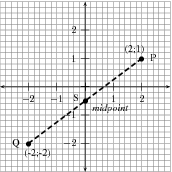
\includegraphics{col11306.imgs/m39119_MG10C14_020.png} % m39119;MG10C14\_020.png;;;6.0;8.5;
        
      \vspace{2pt}
    \vspace{.1in}
    \rule[.1in]{\figurerulewidth}{.005in} \\
        
    \end{center}

 \end{figure}   

    \addtocounter{footnote}{-0}
    \label{m39119*eip-891}The following video provides a summary of the midpoint of a line.

    \setcounter{subfigure}{0}


	\begin{figure}[H] % horizontal\label{m39119*uid666}
    
    
    \textnormal{Khan academy video on midpoint of a line}\vspace{.1in} \nopagebreak
  \label{m39119*yt-media2}\label{m39119*yt-video2}
            \raisebox{-5 pt}{ 
\includegraphics[width=0.5cm]{col11306.imgs/summary_www.png}} { (Video:  MG10112 )}
      
      \vspace{2pt}
    \vspace{.1in}
    
    

 \end{figure}   

    \addtocounter{footnote}{-0}
    \par \label{m39119**end}
          
%          \section{ Summary \& Exercises}
%     \nopagebreak
%             \label{m39167} $ \hspace{-5pt}\begin{array}{cccccccccccc}   \end{array} $ \hspace{2 pt}\raisebox{-5 pt}{
\includegraphics[width=0.5cm]{col11306.imgs/summary_www.png}} {(section shortcode: MG10113 )} \par 
%     
%     
%     
    
    
    
  \label{m39167*fs-id5760712}
            \section{ Summary }
            \nopagebreak
            

\label{m39167*fs-id1165371842904}
\label{m39167*eip-966}\begin{itemize}[noitemsep]
            \item Figures can be represented on the Cartesian plane\item The formula for finding the distance between two points is: \label{m39167*eid9734}\nopagebreak\noindent{}\settowidth{\mymathboxwidth}{\begin{equation}
    \mathrm{Distance}=\sqrt{{\left({x}_{1}-{x}_{2}\right)}^{2}+{\left({y}_{1}-{y}_{2}\right)}^{2}}\tag{15.11}
      \end{equation}
    }
    \typeout{Columnwidth = \the\columnwidth}\typeout{math as usual width = \the\mymathboxwidth}
    \ifthenelse{\lengthtest{\mymathboxwidth < \columnwidth}}{% if the math fits, do it again, for real
    \begin{equation}
    \mathrm{Distance}=\sqrt{{\left({x}_{1}-{x}_{2}\right)}^{2}+{\left({y}_{1}-{y}_{2}\right)}^{2}}\tag{15.11}
      \end{equation}
    }{% else, if it doesn't fit
    \setlength{\mymathboxwidth}{\columnwidth}
      \addtolength{\mymathboxwidth}{-48pt}
    \par\vspace{12pt}\noindent\begin{minipage}{\columnwidth}
    \parbox[t]{\mymathboxwidth}{\large\begin{math}
    \mathrm{Distance}=\sqrt{{\left({x}_{1}-{x}_{2}\right)}^{2}+{\left({y}_{1}-{y}_{2}\right)}^{2}}\end{math}}\hfill
    \parbox[t]{48pt}{\raggedleft 
    (15.11)}
    \end{minipage}\vspace{12pt}\par
    }% end of conditional for this bit of math
    \typeout{math as usual width = \the\mymathboxwidth}
    \item The formula for finding the gradient of a line is: \label{m39167*edi6342}\nopagebreak\noindent{}\settowidth{\mymathboxwidth}{\begin{equation}
    \mathrm{Gradient}=\frac{{y}_{2}-{y}_{1}}{{x}_{2}-{x}_{1}}\tag{15.12}
      \end{equation}
    }
    \typeout{Columnwidth = \the\columnwidth}\typeout{math as usual width = \the\mymathboxwidth}
    \ifthenelse{\lengthtest{\mymathboxwidth < \columnwidth}}{% if the math fits, do it again, for real
    \begin{equation}
    \mathrm{Gradient}=\frac{{y}_{2}-{y}_{1}}{{x}_{2}-{x}_{1}}\tag{15.12}
      \end{equation}
    }{% else, if it doesn't fit
    \setlength{\mymathboxwidth}{\columnwidth}
      \addtolength{\mymathboxwidth}{-48pt}
    \par\vspace{12pt}\noindent\begin{minipage}{\columnwidth}
    \parbox[t]{\mymathboxwidth}{\large\begin{math}
    \mathrm{Gradient}=\frac{{y}_{2}-{y}_{1}}{{x}_{2}-{x}_{1}}\end{math}}\hfill
    \parbox[t]{48pt}{\raggedleft 
    (15.12)}
    \end{minipage}\vspace{12pt}\par
    }% end of conditional for this bit of math
    \typeout{math as usual width = \the\mymathboxwidth}
    \item The formula for finding the midpoint between two points is: \label{m39167*eid6743}\nopagebreak\noindent{}\settowidth{\mymathboxwidth}{\begin{equation}
    S\left(\frac{{x}_{1}+{x}_{2}}{2};\frac{{y}_{1}+{y}_{2}}{2}\right)\tag{15.13}
      \end{equation}
    }
    \typeout{Columnwidth = \the\columnwidth}\typeout{math as usual width = \the\mymathboxwidth}
    \ifthenelse{\lengthtest{\mymathboxwidth < \columnwidth}}{% if the math fits, do it again, for real
    \begin{equation}
    S\left(\frac{{x}_{1}+{x}_{2}}{2};\frac{{y}_{1}+{y}_{2}}{2}\right)\tag{15.13}
      \end{equation}
    }{% else, if it doesn't fit
    \setlength{\mymathboxwidth}{\columnwidth}
      \addtolength{\mymathboxwidth}{-48pt}
    \par\vspace{12pt}\noindent\begin{minipage}{\columnwidth}
    \parbox[t]{\mymathboxwidth}{\large\begin{math}
    S\left(\frac{{x}_{1}+{x}_{2}}{2};\frac{{y}_{1}+{y}_{2}}{2}\right)\end{math}}\hfill
    \parbox[t]{48pt}{\raggedleft 
    (15.13)}
    \end{minipage}\vspace{12pt}\par
    }% end of conditional for this bit of math
    \typeout{math as usual width = \the\mymathboxwidth}
    
\item  If two lines are parallel then they will have the same gradient, i.e. \begin{math}{m}_{\mathrm{AB}}={m}_{\mathrm{CD}}\end{math}. If two lines are perpendicular than we have: \begin{math}-\frac{1}{{m}_{\mathrm{AB}}}={m}_{\mathrm{CD}}\end{math}\end{itemize}
        
\par 
\label{m39167*secfhsst!!!underscore!!!id2370}
            \section{ End of Chapter exercises}
            \nopagebreak
            
        \label{m39167*id69671}\begin{enumerate}[noitemsep, label=\textbf{\arabic*}. ] 
            \label{m39167*uid43466}\item 
Represent the following figures on the Cartesian plane: \label{m39167*id6549695}\begin{enumerate}[noitemsep, label=\textbf{\alph*}. ] 
            \label{m39167*uid4746}\item 
Triangle DEF with D(1;2), E(3;2) and F(2;4) 
\label{m39167*uid4548}\item Quadrilateral GHIJ with G(2;-1), H(0;2), I(-2;-2) and J(1;-3)
\label{m39167*uid4549}\item  Quadrilateral MNOP with M(1;1), N(-1;3), O(-2;3) and P(-4;1) 
\label{m39167*uid5450}\item  Quadrilateral WXYZ with W(1;-2), X(-1;-3), Y(2;-4) and Z(3;-2)
\end{enumerate}
                \label{m39167*uid46}\item 
In the diagram given the vertices of a quadrilateral are F(2;0), G(1;5), H(3;7) and I(7;2).

    \setcounter{subfigure}{0}


	\begin{figure}[H] % horizontal\label{m39167*id69688}
    \begin{center}
    \label{m39167*id69688!!!underscore!!!media}\label{m39167*id69688!!!underscore!!!printimage}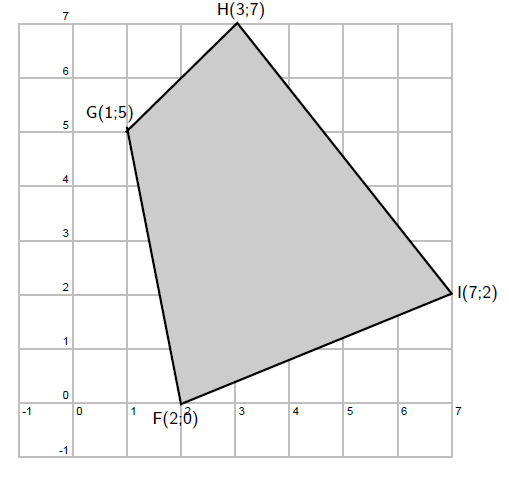
\includegraphics{col11306.imgs/m39167_MG10C14_021.png} % m39167;MG10C14\_021.png;;;6.0;8.5;
        
      \vspace{2pt}
    \vspace{.1in}
    
    \end{center}

 \end{figure}   

    \addtocounter{footnote}{-0}
    \label{m39167*id69695}\begin{enumerate}[noitemsep, label=\textbf{\alph*}. ] 
            \label{m39167*uid47}\item 
What are the lengths of the opposite sides of FGHI?
\label{m39167*uid48}\item Are the opposite sides of FGHI parallel?
\label{m39167*uid49}\item  Do the diagonals of FGHI bisect each other?
\label{m39167*uid50}\item  Can you state what type of quadrilateral FGHI is? Give reasons for your answer.
\end{enumerate}
                \label{m39167*uid51}\item 
A quadrialteral ABCD with vertices A(3;2), B(1;7), C(4;5) and D(1;3) is given.
\label{m39167*id69770}\begin{enumerate}[noitemsep, label=\textbf{\alph*}. ] 
            \label{m39167*uid52}\item  Draw the quadrilateral.
\label{m39167*uid53}\item  Find the lengths of the sides of the quadrilateral.
\end{enumerate}
                \label{m39167*uid54}\item ABCD is a quadrilateral with verticies A(0;3), B(4;3), C(5;-1) and D(-1;-1).
\label{m39167*id69816}\begin{enumerate}[noitemsep, label=\textbf{\alph*}. ] 
            \label{m39167*uid55}\item Show that:
\label{m39167*id69834}\begin{enumerate}[noitemsep, label=\textbf{\roman*}. ] 
            \label{m39167*uid56}\item AD = BC
\label{m39167*uid57}\item AB \begin{math}\^{a}ˆ¥\end{math} DC
\end{enumerate}
        \label{m39167*uid58}\item What name would you give to ABCD?
\label{m39167*uid59}\item Show that the diagonals AC and BD do not bisect each other.
\end{enumerate}
                \label{m39167*uid60}\item P, Q, R and S are the points (-2;0), (2;3), (5;3), (-3;-3) respectively.
\label{m39167*id69919}\begin{enumerate}[noitemsep, label=\textbf{\alph*}. ] 
            \label{m39167*uid61}\item Show that:
\label{m39167*id69937}\begin{enumerate}[noitemsep, label=\textbf{\roman*}. ] 
            \label{m39167*uid62}\item SR = 2PQ
\label{m39167*uid63}\item SR \begin{math}\^{a}ˆ¥\end{math} PQ
\end{enumerate}
        \label{m39167*uid64}\item Calculate:
\label{m39167*id69993}\begin{enumerate}[noitemsep, label=\textbf{\roman*}. ] 
            \label{m39167*uid65}\item PS
\label{m39167*uid66}\item QR
\end{enumerate}
        \label{m39167*uid67}\item What kind of a quadrilateral is PQRS? Give reasons for your answers.
\end{enumerate}
                \label{m39167*uid68}\item EFGH is a parallelogram with verticies E(-1;2), F(-2;-1) and G(2;0). Find the co-ordinates of H by using the fact that the diagonals of a parallelogram bisect each other.\newline
            
\item  
PQRS is a quadrilateral with points P(0; \^{a}ˆ'3) ; Q(\^{a}ˆ'2;5) ; R(3;2) and S(3;\^{a}€``2)  in the Cartesian plane.
\label{m39167*id0812312}\begin{enumerate}[noitemsep, label=\textbf{\alph*}. ] 
            \label{m39167*id08123}\item Find the length of QR.\label{m39167*id981221}\item Find the gradient of PS.\label{m39167*id08213}\item Find the midpoint of PR.\label{m39167*id9871293}\item Is PQRS a parallelogram?  Give reasons for your answer. \end{enumerate}
                \item A(\^{a}€``2;3) and B(2;6) are points in the Cartesian plane.  C(a;b) is the midpoint of AB. Find the values of a and b.\newline
            
\item 
Consider: Triangle ABC with vertices A (1; 3) B (4; 1) and C (6; 4):
\label{m39167*id9173123}\begin{enumerate}[noitemsep, label=\textbf{\alph*}. ] 
            \item Sketch triangle ABC on the Cartesian plane. \item Show that ABC is an isoceles triangle.\item Determine the co-ordinates of M, the midpoint of AC.\item Determine the gradient of AB.\item Show that the following points are collinear: A, B and D(7;-1)\end{enumerate}
                
\item In the diagram, A is the point (-6;1) and B is the point (0;3)

    \setcounter{subfigure}{0}


	\begin{figure}[H] % horizontal\label{m39167*id740344}
    \begin{center}
    \label{m39167*id740344!!!underscore!!!media}\label{m39167*id740344!!!underscore!!!printimage}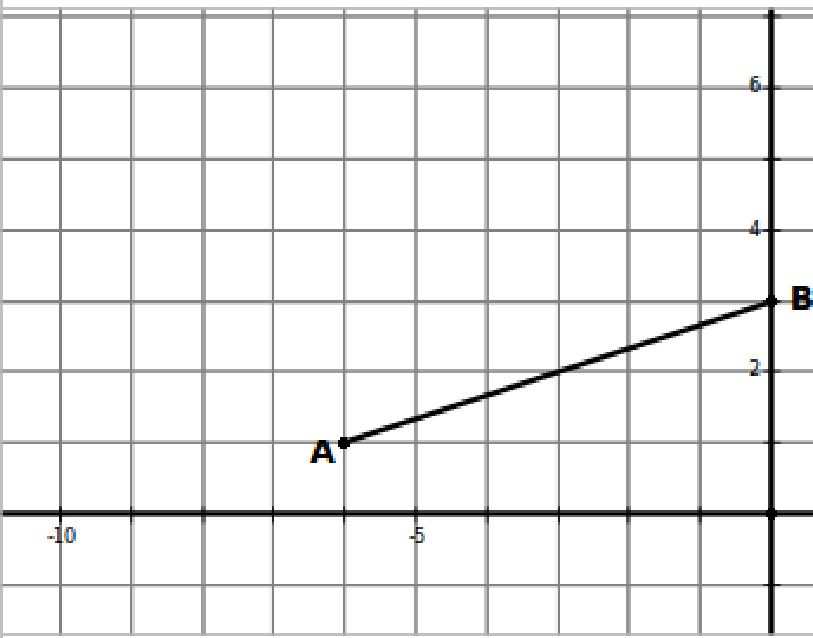
\includegraphics{col11306.imgs/m39167_MG10C14_5.png} % m39167;MG10C14\_5.png;;;6.0;8.5;
        
      \vspace{2pt}
    \vspace{.1in}
    
    \end{center}

 \end{figure}   

    \addtocounter{footnote}{-0}
    \label{m39167*id982373}\begin{enumerate}[noitemsep, label=\textbf{\alph*}. ] 
            \item Find the equation of line AB \item Calculate the length of AB\item  A\^{a}€™ is the image of A and B\^{a}€™ is the image of B. Both these images are obtain by applying the transformation: (x;y)\begin{math}\^{a}†'\end{math}(x-4;y-1). Give the coordinates of both A\^{a}€™ and B\^{a}€™\item Find the equation of A\^{a}€™B\^{a}€™\item Calculate the length of A\^{a}€™B\^{a}€™\item Can you state with certainty that AA'B'B is a parallelogram? Justify your answer.\end{enumerate}
                 \end{enumerate}
        
        

      
\label{m39167**end}
          
       
    
  \label{71522cd1c95e0cbedb9f300409036b1b**end}
    
\par \raisebox{-5 pt}{
\includegraphics[width=0.5cm]{col11306.imgs/summary_www.png}} Find the answers with the shortcodes:
 \par \begin{tabular}[h]{cccccc}
 (1.) lgv  &  (2.) liZ  &  (3.) liB  &  (4.) lac  &  (5.) lax  &  (6.) laa  &  (7.) laY  &  (8.) lag  &  (9.) la4  &  (10.) l4o  & \end{tabular}



